\documentclass{standalone}

\usepackage{import}
\subimport{../../../}{preamble.tex}

\usepackage{tikz}
\usetikzlibrary{arrows}
\usetikzlibrary{decorations.pathreplacing}

\begin{document}
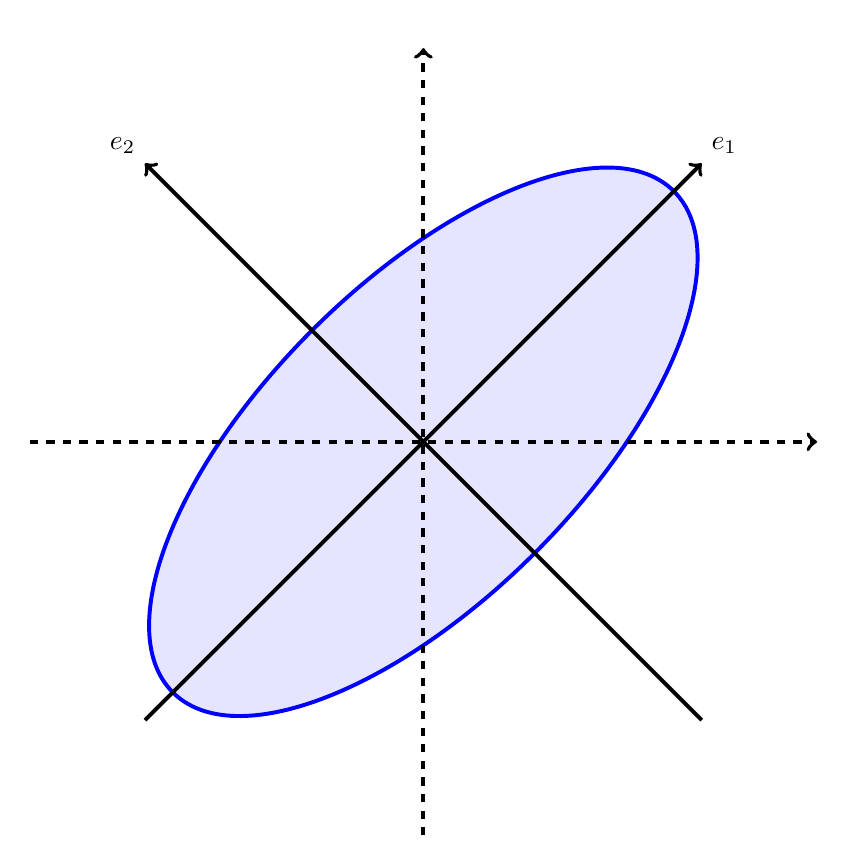
\begin{tikzpicture}
\begin{scope}[remember picture,rotate=45]
    \coordinate (O) at (0,0);
    \coordinate (A) at (4.5,0);
    \coordinate (B) at (0,2);
    % draw ellipse
    \draw[line width = 0.5mm, blue, fill=blue!10] (O) ellipse (4.5cm and 2.0cm);
    % draw axis
    \draw[line width = 0.5mm, ->] (-5, 0) -- (5, 0) coordinate[right] (e1);
    \draw[line width = 0.5mm, ->] (0, -5) -- (0, 5) coordinate[above] (e2);
    % calculate brace points for major axis
    \path (O) -- (A) coordinate[pos=.02] (a1) coordinate[pos=.98] (a2);
    %\draw[decorate, decoration = {brace, amplitude = 15pt, mirror, raise =4pt}, yshift = 0pt]
        (a2) -- (a1) coordinate[midway] (tl1);
    %\coordinate (l1) at ([yshift=1cm]tl1);
    % calculate brace points for minor axis
    \path (O) -- (B) coordinate[pos=.05] (b1) coordinate[pos=.95] (b2);
    %\draw[decorate, decoration = {brace, amplitude = 15pt, mirror, raise =4pt}, yshift = 0pt]
    %    (b2) -- (b1) coordinate[midway] (tl2);
    %\coordinate (l2) at ([xshift=-.9cm]tl2);
\end{scope}
\draw[line width = 0.5mm, dashed, ->] (-5, 0) -- (5, 0) node[right]{};
\draw[line width = 0.5mm, dashed, ->] (0, -5) -- (0, 5) node[above]{};
\node[anchor=south west] at (e1) {$e_1$};
\node[anchor=south east] at (e2) {$e_2$};
% \node[anchor=south west] at (l1) {$\frac{c}{\sqrt{\lambda_1}}$};
% \node[anchor=south east] at ([xshift=.1cm]l2) {$\frac{c}{\sqrt{\lambda_2}}$};   
\end{tikzpicture}
\end{document}
%%% Local Variables:
%%% mode: latex
%%% TeX-master: t
%%% End:
